% ============================================================
% Pantry Dashboard v2 — Beamer Presentation
% Engine: LuaLaTeX
% Theme: Custom (warm cream + sage green)
% ============================================================
\documentclass[aspectratio=169,12pt]{beamer}

% ── Fonts & encoding ─────────────────────────────────────────
\usepackage{fontspec}
\setmainfont{TeX Gyre Heros}
\setsansfont{TeX Gyre Heros}
\setmonofont{DejaVu Sans Mono}[Scale=0.85]

% ── Core packages ────────────────────────────────────────────
\usepackage{graphicx}
\usepackage{booktabs}
\usepackage{colortbl}
\usepackage{xcolor}
\usepackage{tikz}
\usepackage{pgfplots}
\pgfplotsset{compat=1.18}
\usepackage{microtype}
\usepackage{array}
\usepackage{tabularx}
\usepackage{enumitem}
\usepackage{adjustbox}
\usepackage{tcolorbox}
\tcbuselibrary{skins,breakable}

% ── Color palette (from spec) ────────────────────────────────
\definecolor{cream}{HTML}{FEFCF3}
\definecolor{cardBg}{HTML}{F5EFD8}
\definecolor{sage}{HTML}{5B8C5A}
\definecolor{sageDark}{HTML}{4A7249}
\definecolor{warmGray}{HTML}{8B956D}
\definecolor{bodyText}{HTML}{2C2C2C}
\definecolor{muted}{HTML}{9B9B7A}
\definecolor{accent}{HTML}{D4A843}
\definecolor{errRed}{HTML}{C0392B}
\definecolor{infoBlue}{HTML}{4A90D9}

% Category colors
\definecolor{catDairy}{HTML}{4A90D9}
\definecolor{catProduce}{HTML}{7CB87A}
\definecolor{catMeat}{HTML}{E07B54}
\definecolor{catGrains}{HTML}{D4A843}
\definecolor{catSnacks}{HTML}{9B59B6}
\definecolor{catCond}{HTML}{E67E22}
\definecolor{catFrozen}{HTML}{5DADE2}
\definecolor{catBev}{HTML}{58D68D}
\definecolor{catMeals}{HTML}{EC407A}
\definecolor{catOther}{HTML}{95A5A6}

% ── Beamer theme setup ───────────────────────────────────────
\usetheme{default}
\usecolortheme{default}
\usefonttheme{professionalfonts}

% Background
\setbeamercolor{background canvas}{bg=cream}

% Frame title
\setbeamercolor{frametitle}{fg=bodyText,bg=cardBg}
\setbeamerfont{frametitle}{size=\large,series=\bfseries}
\setbeamertemplate{frametitle}{%
  \vspace{0.15cm}%
  \hspace{0.3cm}%
  
\begin{tikzpicture}[overlay,remember picture]
    \fill[sage] (0, -0.05) rectangle (-0.18, 0.55);
  \end{tikzpicture}%
  \hspace{0.25cm}\insertframetitle
  \vspace{0.1cm}%
}

% Footer
\setbeamercolor{footline}{fg=muted,bg=cardBg}
\setbeamertemplate{footline}{%
  \leavevmode%
  \hbox{%
    \begin{beamercolorbox}[wd=0.5\paperwidth,ht=2.2ex,dp=1ex,left]{footline}%
      \hspace{0.4cm}\small\color{muted}Pantry Dashboard v2
    \end{beamercolorbox}%
    \begin{beamercolorbox}[wd=0.5\paperwidth,ht=2.2ex,dp=1ex,right]{footline}%
      \small\color{muted}\insertframenumber{} / \inserttotalframenumber\hspace{0.4cm}
    \end{beamercolorbox}%
  }%
}

% Navigation: off
\setbeamertemplate{navigation symbols}{}

% Items
\setbeamercolor{item}{fg=sage}
\setbeamercolor{subitem}{fg=warmGray}
\setbeamertemplate{itemize item}{\color{sage}\textbullet}
\setbeamertemplate{itemize subitem}{\color{warmGray}\textendash}
\setbeamerfont{itemize/enumerate body}{size=\small}
\setbeamerfont{itemize/enumerate subbody}{size=\footnotesize}

% Blocks
\setbeamercolor{block title}{fg=white,bg=sage}
\setbeamercolor{block body}{fg=bodyText,bg=cardBg}
\setbeamerfont{block title}{size=\small,series=\bfseries}

% Alert block
\setbeamercolor{block title alerted}{fg=white,bg=errRed}
\setbeamercolor{block alerted body}{fg=bodyText,bg=cream}

% Example block
\setbeamercolor{block title example}{fg=white,bg=infoBlue}
\setbeamercolor{block body example}{fg=bodyText,bg=cream}

% Captions
\setbeamercolor{caption name}{fg=muted}
\setbeamerfont{caption}{size=\tiny}

% ── Helper macros ────────────────────────────────────────────
\newcommand{\pill}[2]{%
  \tikz[baseline=(t.base)]\node[draw=#1,fill=#1!15,rounded corners=3pt,
    inner sep=2pt,text=#1,font=\tiny\bfseries](t){#2};%
}
\newcommand{\codebox}[1]{%
  \colorbox{cardBg}{\small\ttfamily #1}%
}
\newcommand{\spec}[1]{\textcolor{sage}{\textbf{#1}}}
\newcommand{\warn}[1]{\textcolor{accent}{\textbf{#1}}}
\newcommand{\bad}[1]{\textcolor{errRed}{\textbf{#1}}}

% ── tcolorbox styles ─────────────────────────────────────────
\tcbset{
  pantrybox/.style={
    colback=cardBg, colframe=sage, coltext=bodyText,
    boxrule=0.8pt, arc=4pt, left=6pt, right=6pt, top=4pt, bottom=4pt,
    fonttitle=\small\bfseries, coltitle=bodyText, attach boxed title to top left,
    boxed title style={colback=sage,colframe=sage,arc=3pt,
      fontupper=\small\bfseries\color{white},boxrule=0pt}
  },
  statcard/.style={
    colback=cream, colframe=#1, coltext=bodyText,
    boxrule=1.5pt, arc=5pt, left=5pt, right=5pt, top=4pt, bottom=4pt,
    width=0.22\textwidth, nobeforeafter, box align=top
  },
}

% ────────────────────────────────────────────────────────────
\begin{document}

% ── TITLE SLIDE ─────────────────────────────────────────────
{
\setbeamertemplate{footline}{}
\setbeamertemplate{frametitle}{}
\begin{frame}[plain]
  \begin{tikzpicture}[remember picture,overlay]
    % Background
    \fill[cream] (current page.south west) rectangle (current page.north east);
    % Sage accent bar left
    \fill[sage] (current page.south west) ++(-0.1,-0.1) rectangle ++(0.6,10);
    % Subtle grid pattern (decorative)
    \foreach \y in {0,0.8,...,8}{
      \draw[cardBg,line width=0.4pt] (current page.south west) ++(0.6,\y)
        -- ++(16,0);
    }
    % Card
    \fill[cardBg,rounded corners=8pt]
      (current page.center) ++(-5.5,-2.5) rectangle ++(11,5);
    \draw[sage,line width=1pt,rounded corners=8pt]
      (current page.center) ++(-5.5,-2.5) rectangle ++(11,5);
  \end{tikzpicture}

  \vspace{2.2cm}
  \begin{center}
    {\color{sage}\rule{2cm}{2pt}}\\[0.3cm]
    {\Huge\bfseries\color{bodyText} Pantry Dashboard v2}\\[0.4cm]
    {\large\color{warmGray} From stretched mobile to a warm, intelligent pantry system}\\[0.6cm]
    {\small\color{muted} Cyrus Dioun \quad\textperiodcentered\quad March 2026}\\[0.3cm]
    {\color{sage}\rule{2cm}{2pt}}
  \end{center}
\end{frame}
}

% ── SLIDE 2: THE PROBLEM ────────────────────────────────────
\begin{frame}[t,shrink=25]{The Problem — v1 Limitations}
  \begin{columns}[T]
    \column{0.52\textwidth}
      \begin{tcolorbox}[pantrybox,title={v1 Audit Summary}]
        {\footnotesize
        \begin{itemize}[leftmargin=*,itemsep=2pt]
          \item[\textcolor{errRed}{\textbullet}] \bad{No category system} ---
            38/58 products have OFF data, unused
          \item[\textcolor{errRed}{\textbullet}] \bad{Desktop is stretched mobile} ---
            no sidebar, no desktop layout
          \item[\textcolor{errRed}{\textbullet}] \bad{Bare empty/error states} ---
            no retry, no skeleton loading
          \item[\textcolor{accent}{\textbullet}] \warn{Location cycling hidden} ---
            blind tap-to-rotate, no dropdown
          \item[\textcolor{accent}{\textbullet}] \warn{Sort direction missing} ---
            A\textrightarrow Z vs Z\textrightarrow A unclear
          \item[\textcolor{sage}{\textbullet}] \spec{Kept:} warm palette, emoji system, expiry urgency
        \end{itemize}
        }
      \end{tcolorbox}

    \column{0.45\textwidth}
      \begin{center}
        \includegraphics[width=0.95\textwidth,height=4.5cm,keepaspectratio]%
          {figures/v1-desktop.png}\\[0.1cm]
        {\tiny\color{muted} v1 desktop: stretched card grid, no sidebar,
          no category filters}
      \end{center}
  \end{columns}
\end{frame}

% ── SLIDE 3: DESIGN PROCESS ─────────────────────────────────
\begin{frame}[t,shrink=25]{Design Process — Three Concepts Evaluated}
  \begin{columns}[T]
    \column{0.48\textwidth}
      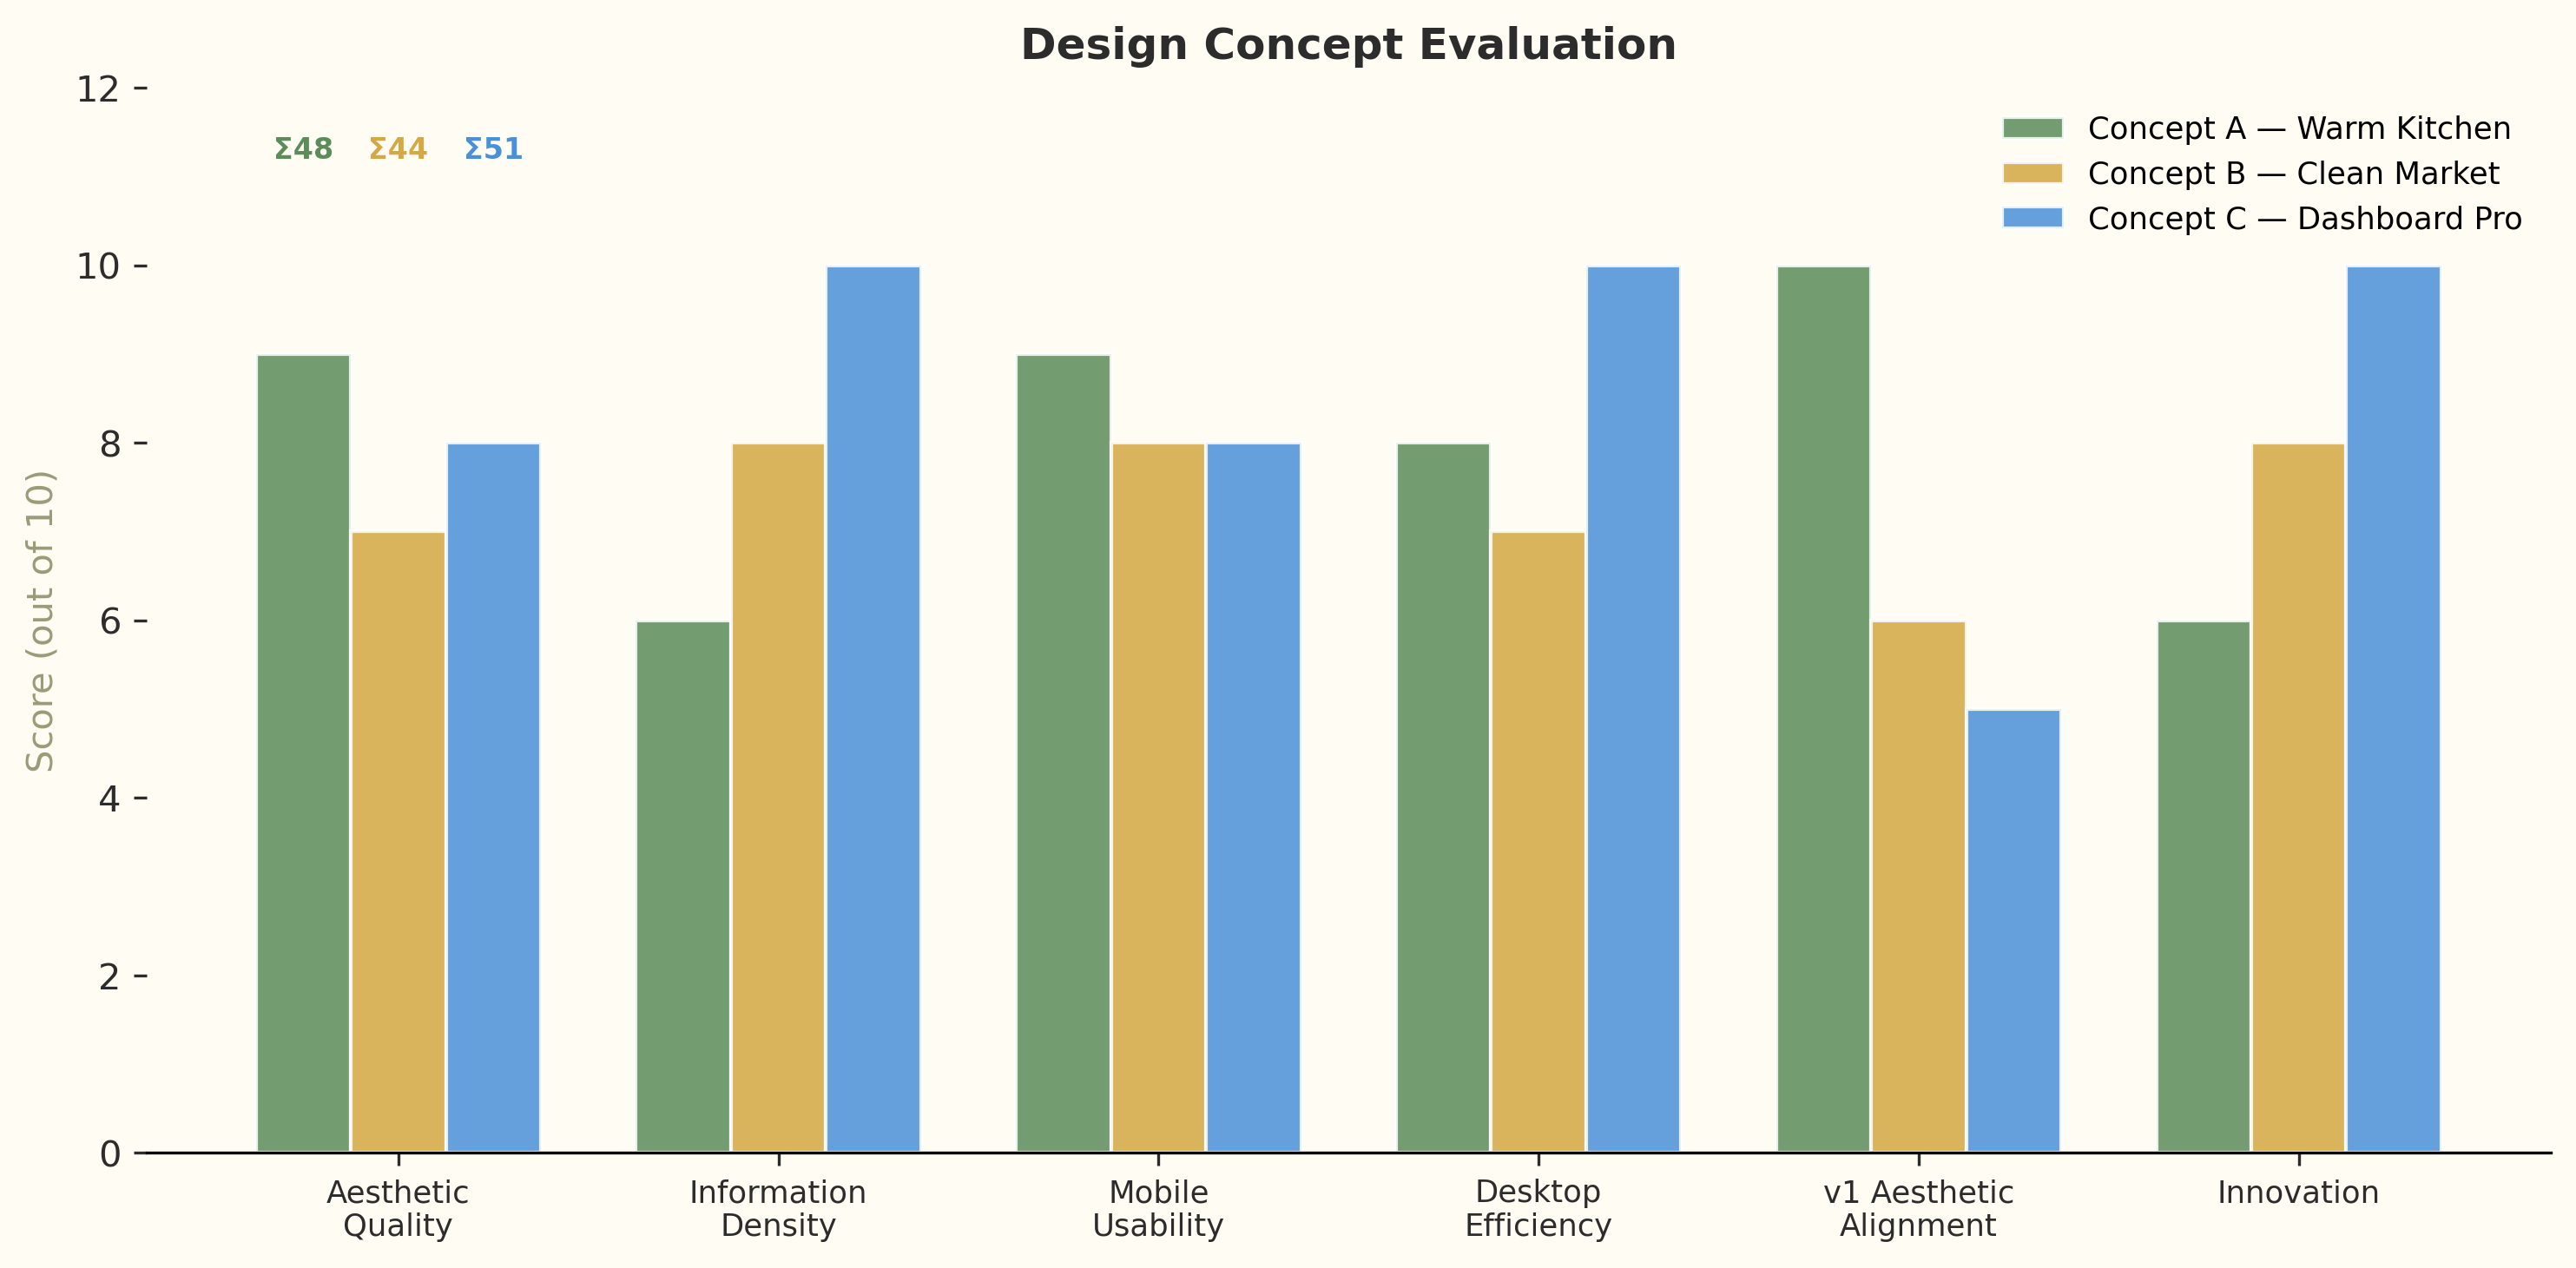
\includegraphics[width=\textwidth]{figures/design_scoring.png}\\[0.2cm]
      \begin{tcolorbox}[colback=cardBg,colframe=sage,boxrule=0.6pt,arc=3pt,
          left=4pt,right=4pt,top=2pt,bottom=2pt]
        {\small\bfseries Decision:} \textbf{A + C Hybrid} (``Warm Dashboard'')\\[1pt]
        {\scriptsize\color{warmGray}
          \textbf{A:} cream/sage palette, cards, pill scroll\quad
          \textbf{C:} sidebar, stat cards, sort direction\\
          \textbf{Not C's dark sidebar} --- too clinical for a kitchen app
        }
      \end{tcolorbox}

    \column{0.49\textwidth}
      \vspace{-0.2cm}
      \begin{center}
        \includegraphics[width=0.85\textwidth,height=2.1cm,keepaspectratio]%
          {figures/concept-a-desktop.png}\\
        {\tiny\color{muted} Concept A --- Warm Kitchen}\\[0.15cm]
        \includegraphics[width=0.85\textwidth,height=2.1cm,keepaspectratio]%
          {figures/concept-c-desktop.png}\\
        {\tiny\color{muted} Concept C --- Dashboard Pro (structure adopted, dark sidebar rejected)}
      \end{center}
  \end{columns}
\end{frame}

% ── SLIDE 4: ARCHITECTURE ───────────────────────────────────
\begin{frame}[t,shrink=25]{Architecture — Data Flow}
  \begin{center}
    \includegraphics[width=0.95\textwidth,height=4.2cm,keepaspectratio]%
      {figures/architecture.png}
  \end{center}
  \vspace{0.1cm}
  \begin{columns}[T]
    \column{0.33\textwidth}
      \begin{block}{Scan Pipeline}
        {\scriptsize
        Photo \textrightarrow{} Dropbox \textrightarrow{} \codebox{scan.py}
        \textrightarrow{} OFF lookup \textrightarrow{} cat mapper
        \textrightarrow{} \codebox{inventory.json}
        }
      \end{block}
    \column{0.33\textwidth}
      \begin{block}{Dashboard Stack}
        {\scriptsize
        Single-file HTML + vanilla JS\\
        Python server at \codebox{:9002}\\
        60s auto-refresh poll
        }
      \end{block}
    \column{0.31\textwidth}
      \begin{block}{API Endpoints}
        {\scriptsize\ttfamily
        GET /api/pantry\\
        PATCH /api/pantry/<bc>\\
        POST /api/pantry\\
        DELETE /api/pantry/<bc>
        }
      \end{block}
  \end{columns}
\end{frame}

% ── SLIDE 5: CATEGORY SYSTEM ────────────────────────────────
\begin{frame}[t,shrink=25]{Category System — 10 Pantry Categories}
  \begin{columns}[T]
    \column{0.42\textwidth}
      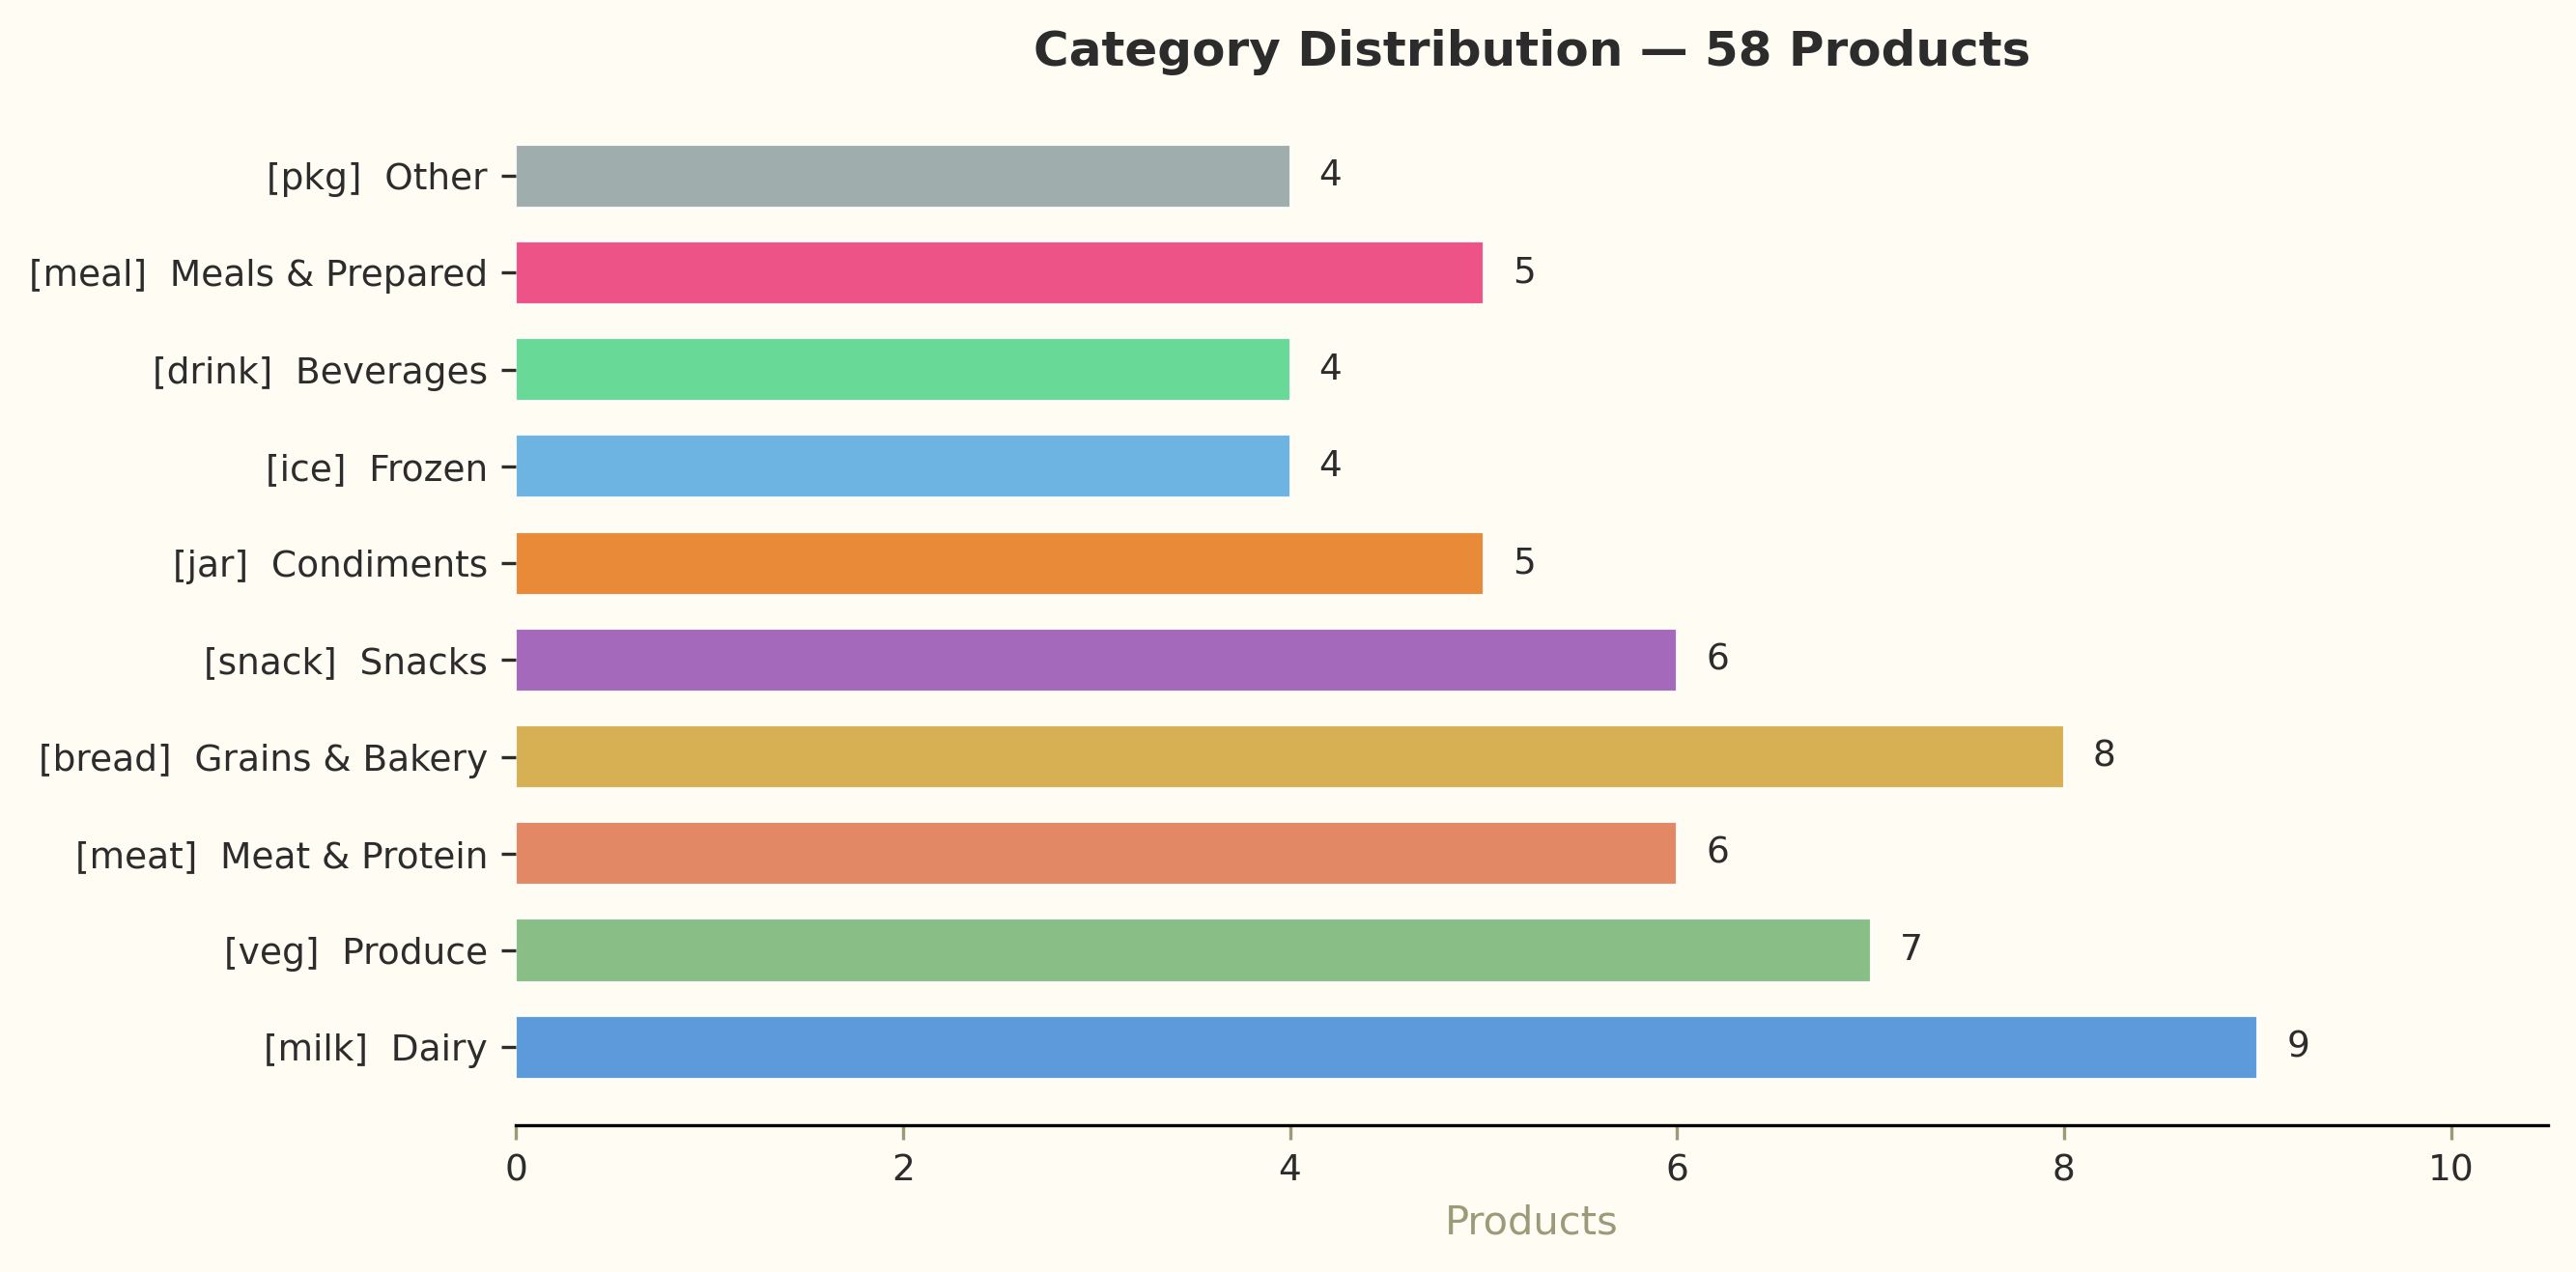
\includegraphics[width=\textwidth]{figures/category_dist.png}

    \column{0.55\textwidth}
      \vspace{-0.1cm}
      \begin{tcolorbox}[pantrybox,title={Mapping Logic}]
        {\footnotesize
        \begin{enumerate}[leftmargin=*,itemsep=2pt,label=\textbf{\arabic*.}]
          \item Take \codebox{categories} string from OFF\\
                (e.g.\ \textit{``Dairies, Milks, Cow milks''})
          \item Split by comma, check each segment\\
                against keyword table
          \item First match wins (most specific)
          \item No match or empty \textrightarrow{} ``Other''
        \end{enumerate}
        }
      \end{tcolorbox}
      \vspace{0.2cm}
      \begin{tcolorbox}[pantrybox,title={Persistence}]
        {\footnotesize
        \codebox{category\_source: "auto"} --- re-scan can update\\[2pt]
        \codebox{category\_source: "manual"} --- user override\\ preserved across all future scans
        }
      \end{tcolorbox}
      \vspace{0.2cm}
      {\footnotesize\color{warmGray}
        38/58 products had OFF taxonomy data \textrightarrow{} auto-mapped.\\
        Remainder assigned ``Other'' and manually corrected.
      }
  \end{columns}
\end{frame}

% ── SLIDE 6: CATEGORY UI ────────────────────────────────────
\begin{frame}[t,shrink=25]{Category UI --- Filter Pills, Badges, Dropdown}
  \begin{columns}[T]
    \column{0.50\textwidth}
      \vspace{-0.1cm}
      \includegraphics[width=\textwidth,height=3.2cm,keepaspectratio]%
        {figures/phase2-mobile.png}\\[0.05cm]
      {\tiny\color{muted} Mobile: horizontal pill scroll with emoji + name + count}\\[0.25cm]
      \includegraphics[width=\textwidth,height=2.4cm,keepaspectratio]%
        {figures/category-dropdown.png}\\[0.05cm]
      {\tiny\color{muted} Category dropdown picker (replaces blind cycling)}

    \column{0.47\textwidth}
      \begin{tcolorbox}[pantrybox,title={Three-layer Filtering}]
        {\footnotesize
        \begin{itemize}[leftmargin=*,itemsep=4pt]
          \item \textbf{Location} --- Pantry / Fridge / Freezer / Spice Rack
          \item \textbf{Category} --- pill bar (10 categories + All)
          \item \textbf{Search} --- text substring match
        \end{itemize}
        \vspace{4pt}
        All three stack: e.g.\ \textit{Fridge + Dairy + ``organic''} shows only
        organic dairy items in the fridge.
        }
      \end{tcolorbox}
      \vspace{0.2cm}
      \begin{tcolorbox}[pantrybox,title={Card Badge}]
        {\footnotesize
        Each card shows a colored pill:\\[3pt]
        \pill{catDairy}{Dairy}~
        \pill{catProduce}{Produce}~
        \pill{catMeat}{Meat}~
        \pill{catGrains}{Grains}\\[4pt]
        \pill{catSnacks}{Snacks}~
        \pill{catFrozen}{Frozen}~
        \pill{catBev}{Beverages}~
        \pill{catMeals}{Meals}\\[4pt]
        Tap badge \textrightarrow{} dropdown to override category
        }
      \end{tcolorbox}
  \end{columns}
\end{frame}

% ── SLIDE 7: DESKTOP LAYOUT ─────────────────────────────────
\begin{frame}[t,shrink=25]{Desktop Layout --- Sidebar Overhaul}
  \begin{columns}[T]
    \column{0.50\textwidth}
      \begin{center}
        {\small\bfseries\color{errRed} Before (v1)}\\[0.2cm]
        \includegraphics[width=0.95\textwidth,height=3.2cm,keepaspectratio]%
          {figures/v1-desktop.png}\\
        {\tiny\color{muted} Stretched mobile layout at 1200px}
      \end{center}

    \column{0.47\textwidth}
      \begin{center}
        {\small\bfseries\color{sage} After (v2)}\\[0.2cm]
        \includegraphics[width=0.95\textwidth,height=3.2cm,keepaspectratio]%
          {figures/phase3-desktop.png}\\
        {\tiny\color{muted} 280px sticky sidebar + 2--3 column card grid}
      \end{center}
  \end{columns}
  \vspace{0.25cm}
  \begin{columns}[T]
    \column{0.32\textwidth}
      \begin{block}{Sidebar (>1024px)}
        {\footnotesize Stat cards \textrightarrow{} location list \textrightarrow{} category
        filters \textrightarrow{} sort controls. Background: \codebox{\#F8F4EC}}
      \end{block}
    \column{0.32\textwidth}
      \begin{block}{Tablet (600--1024px)}
        {\footnotesize Hamburger icon \textrightarrow{} slide-in sidebar overlay.
        Preserves mobile pill UX.}
      \end{block}
    \column{0.32\textwidth}
      \begin{block}{Mobile (<600px)}
        {\footnotesize Single column. Location tabs + category pill scroll.
        No sidebar. Zero regression from v1.}
      \end{block}
  \end{columns}
\end{frame}

% ── SLIDE 8: POLISH FEATURES ────────────────────────────────
\begin{frame}[t,shrink=25]{Polish Features --- Every Edge Case Handled}
  \begin{columns}[T]
    \column{0.48\textwidth}
      \vspace{-0.1cm}
      \begin{tcolorbox}[pantrybox,title={States}]
        {\footnotesize
        \begin{itemize}[leftmargin=*,itemsep=3pt]
          \item \textbf{Loading} --- skeleton shimmer cards (gray animated rectangles in grid)
          \item \textbf{Empty} --- centered illustration + ``Your pantry is empty'' + Add CTA
          \item \textbf{Error} --- warm amber tone, Retry button calls \codebox{loadPantry()} directly
          \item \textbf{Out of stock} --- qty=0 \textrightarrow{} \pill{errRed}{Out of stock} badge + muted card
        \end{itemize}
        }
      \end{tcolorbox}
      \vspace{0.2cm}
      \begin{tcolorbox}[pantrybox,title={Interaction Fixes}]
        {\footnotesize
        \begin{itemize}[leftmargin=*,itemsep=3pt]
          \item Location: dropdown select (not blind cycle)
          \item Sort: \textbf{\textcolor{sage}{A\textrightarrow{}Z}} / \textbf{\textcolor{sage}{Z\textrightarrow{}A}} direction toggle
          \item Stats as clickable filters (tap ``Expiring'' \textrightarrow{} filter view)
          \item Null nutrition fields hidden (not shown as ``null'')
        \end{itemize}
        }
      \end{tcolorbox}

    \column{0.49\textwidth}
      \vspace{-0.1cm}
      \begin{center}
        \includegraphics[width=0.46\textwidth,height=2.8cm,keepaspectratio]%
          {figures/empty-state.png}%
        \hfill%
        \includegraphics[width=0.46\textwidth,height=2.8cm,keepaspectratio]%
          {figures/error-state.png}\\[0.05cm]
        {\tiny\color{muted} Empty state (left) and error state (right)}\\[0.3cm]
        \includegraphics[width=0.95\textwidth,height=2.4cm,keepaspectratio]%
          {figures/stat-filter.png}\\[0.05cm]
        {\tiny\color{muted} Stats as interactive filters in sidebar}
      \end{center}
  \end{columns}
\end{frame}

% ── SLIDE 9: NUTRITION API RESEARCH ─────────────────────────
\begin{frame}[t,shrink=25]{Nutrition API Research --- Closing Coverage Gaps}
  \begin{columns}[T]
    \column{0.52\textwidth}
      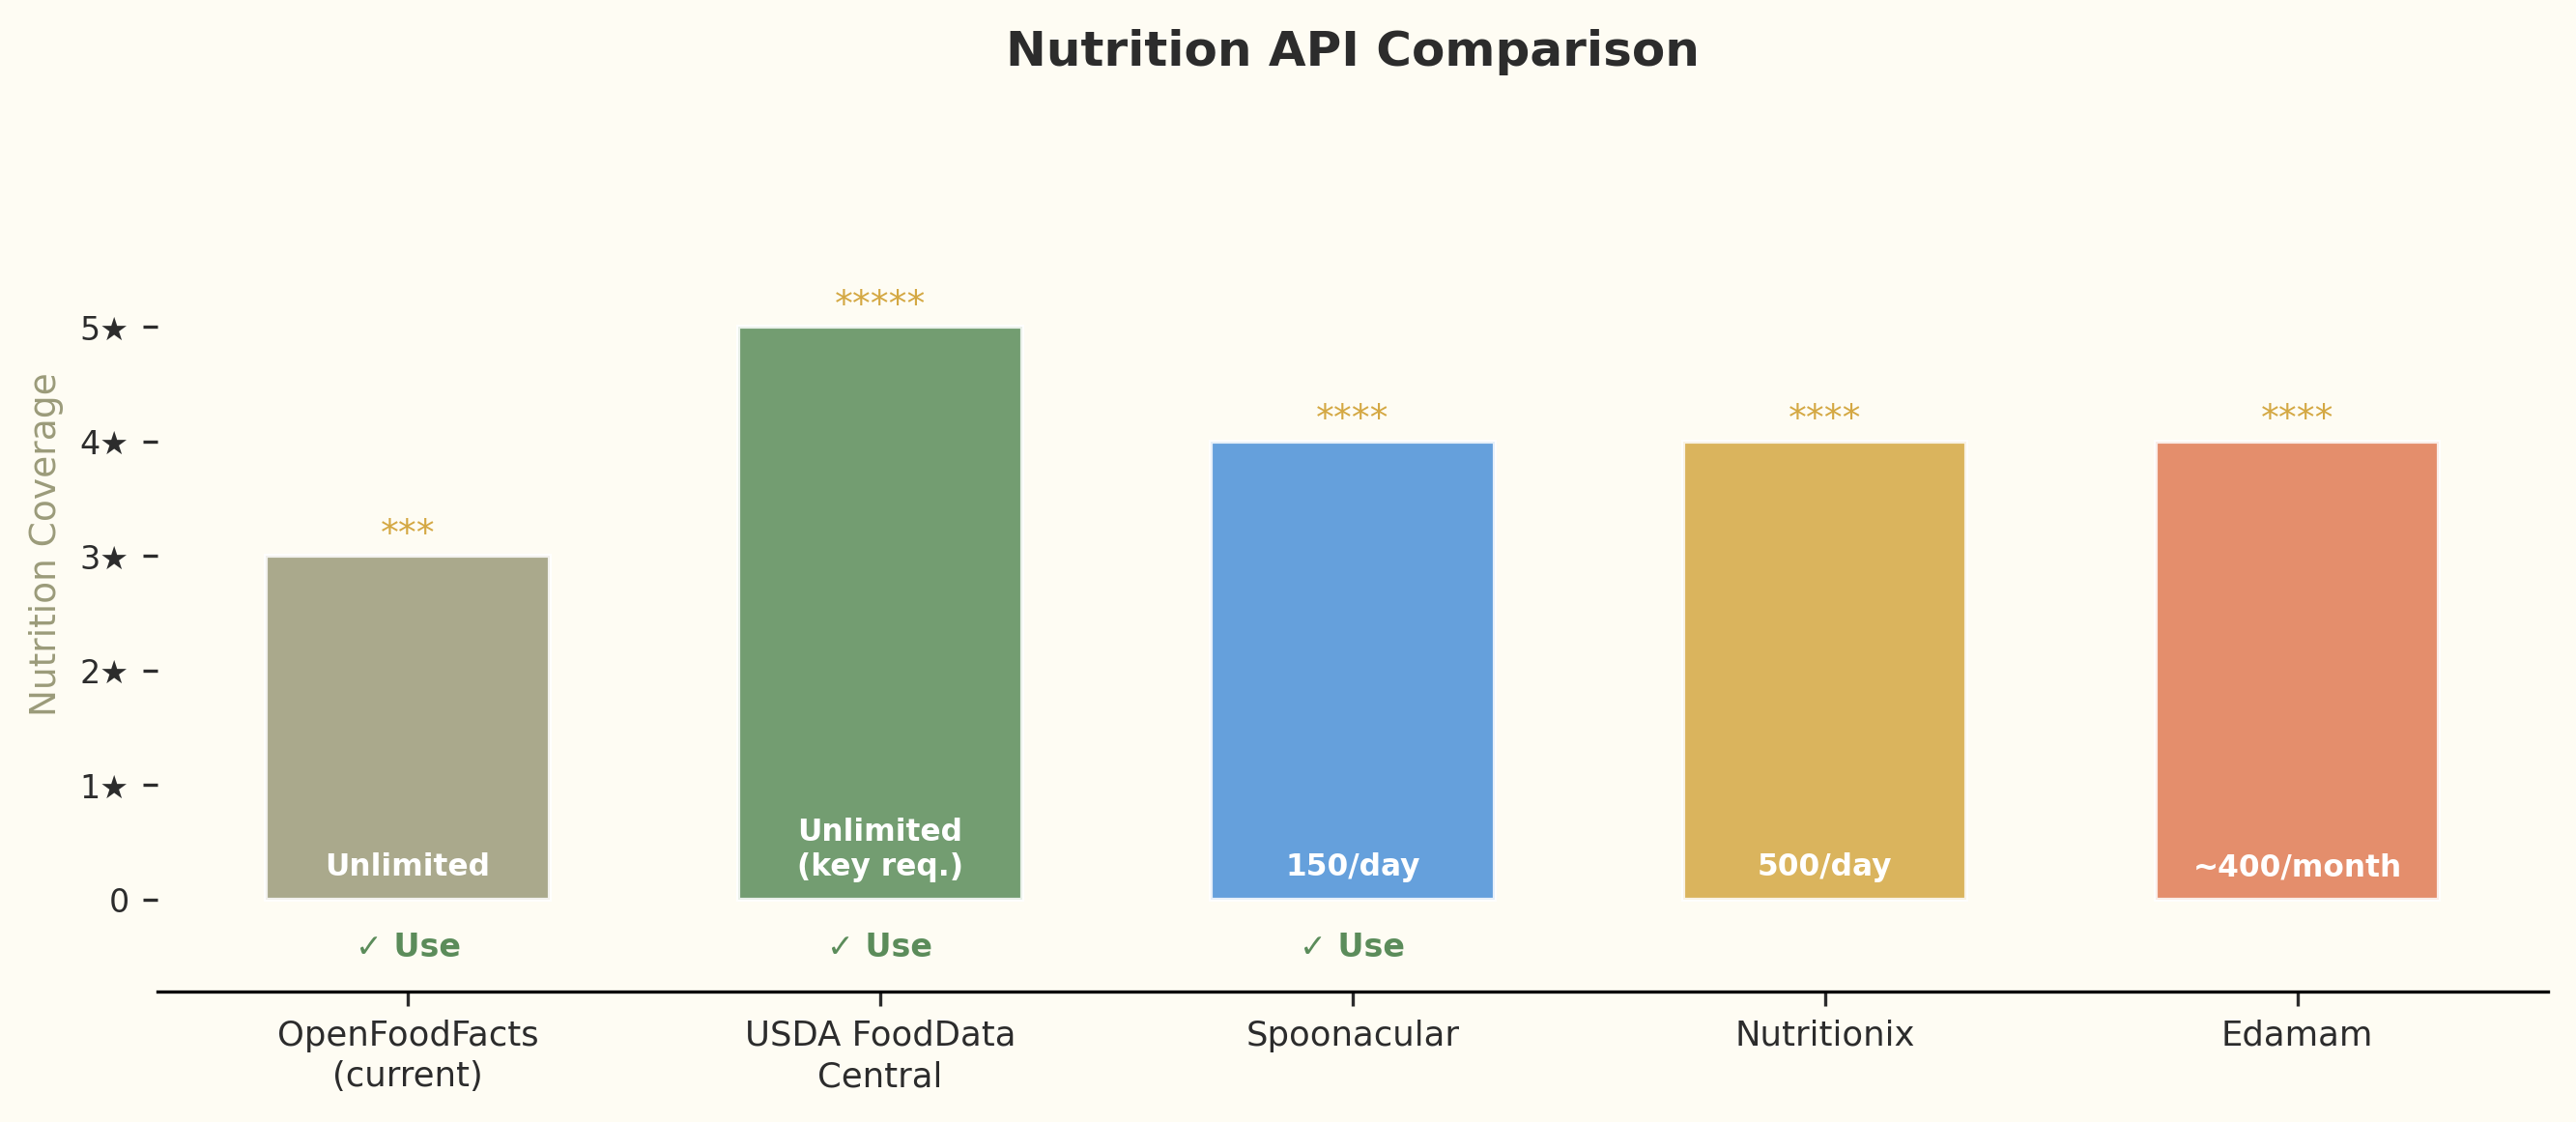
\includegraphics[width=\textwidth]{figures/nutrition_apis.png}

    \column{0.45\textwidth}
      \begin{tcolorbox}[pantrybox,title={Problem}]
        {\footnotesize
        OpenFoodFacts is community-maintained. Many US grocery products
        have sparse nutrition data: calories, fiber, and vitamins frequently null.
        }
      \end{tcolorbox}
      \vspace{0.2cm}
      \begin{tcolorbox}[pantrybox,title={Recommended Fallback Stack}]
        {\footnotesize
        \begin{enumerate}[leftmargin=*,itemsep=3pt,label=\textbf{\arabic*.}]
          \item \spec{OpenFoodFacts} (current, primary) --- best international coverage
          \item \spec{USDA FoodData Central} (fallback 1) --- 100\% free, unlimited,
                lab-validated, 250K branded foods
          \item \spec{Spoonacular} (fallback 2) --- clean UPC endpoint, 150/day free,
                sufficient for household scan volume
        \end{enumerate}
        }
      \end{tcolorbox}
      \vspace{0.05cm}
      {\scriptsize\color{warmGray}
        Skip: Edamam (free tier too restrictive), Nutritionix (redundant with USDA).
      }
  \end{columns}
\end{frame}

% ── SLIDE 10: DESIGN SYSTEM ─────────────────────────────────
\begin{frame}[t,shrink=25]{Design System --- Color Tokens \& Typography}
  \begin{columns}[T]
    \column{0.53\textwidth}
      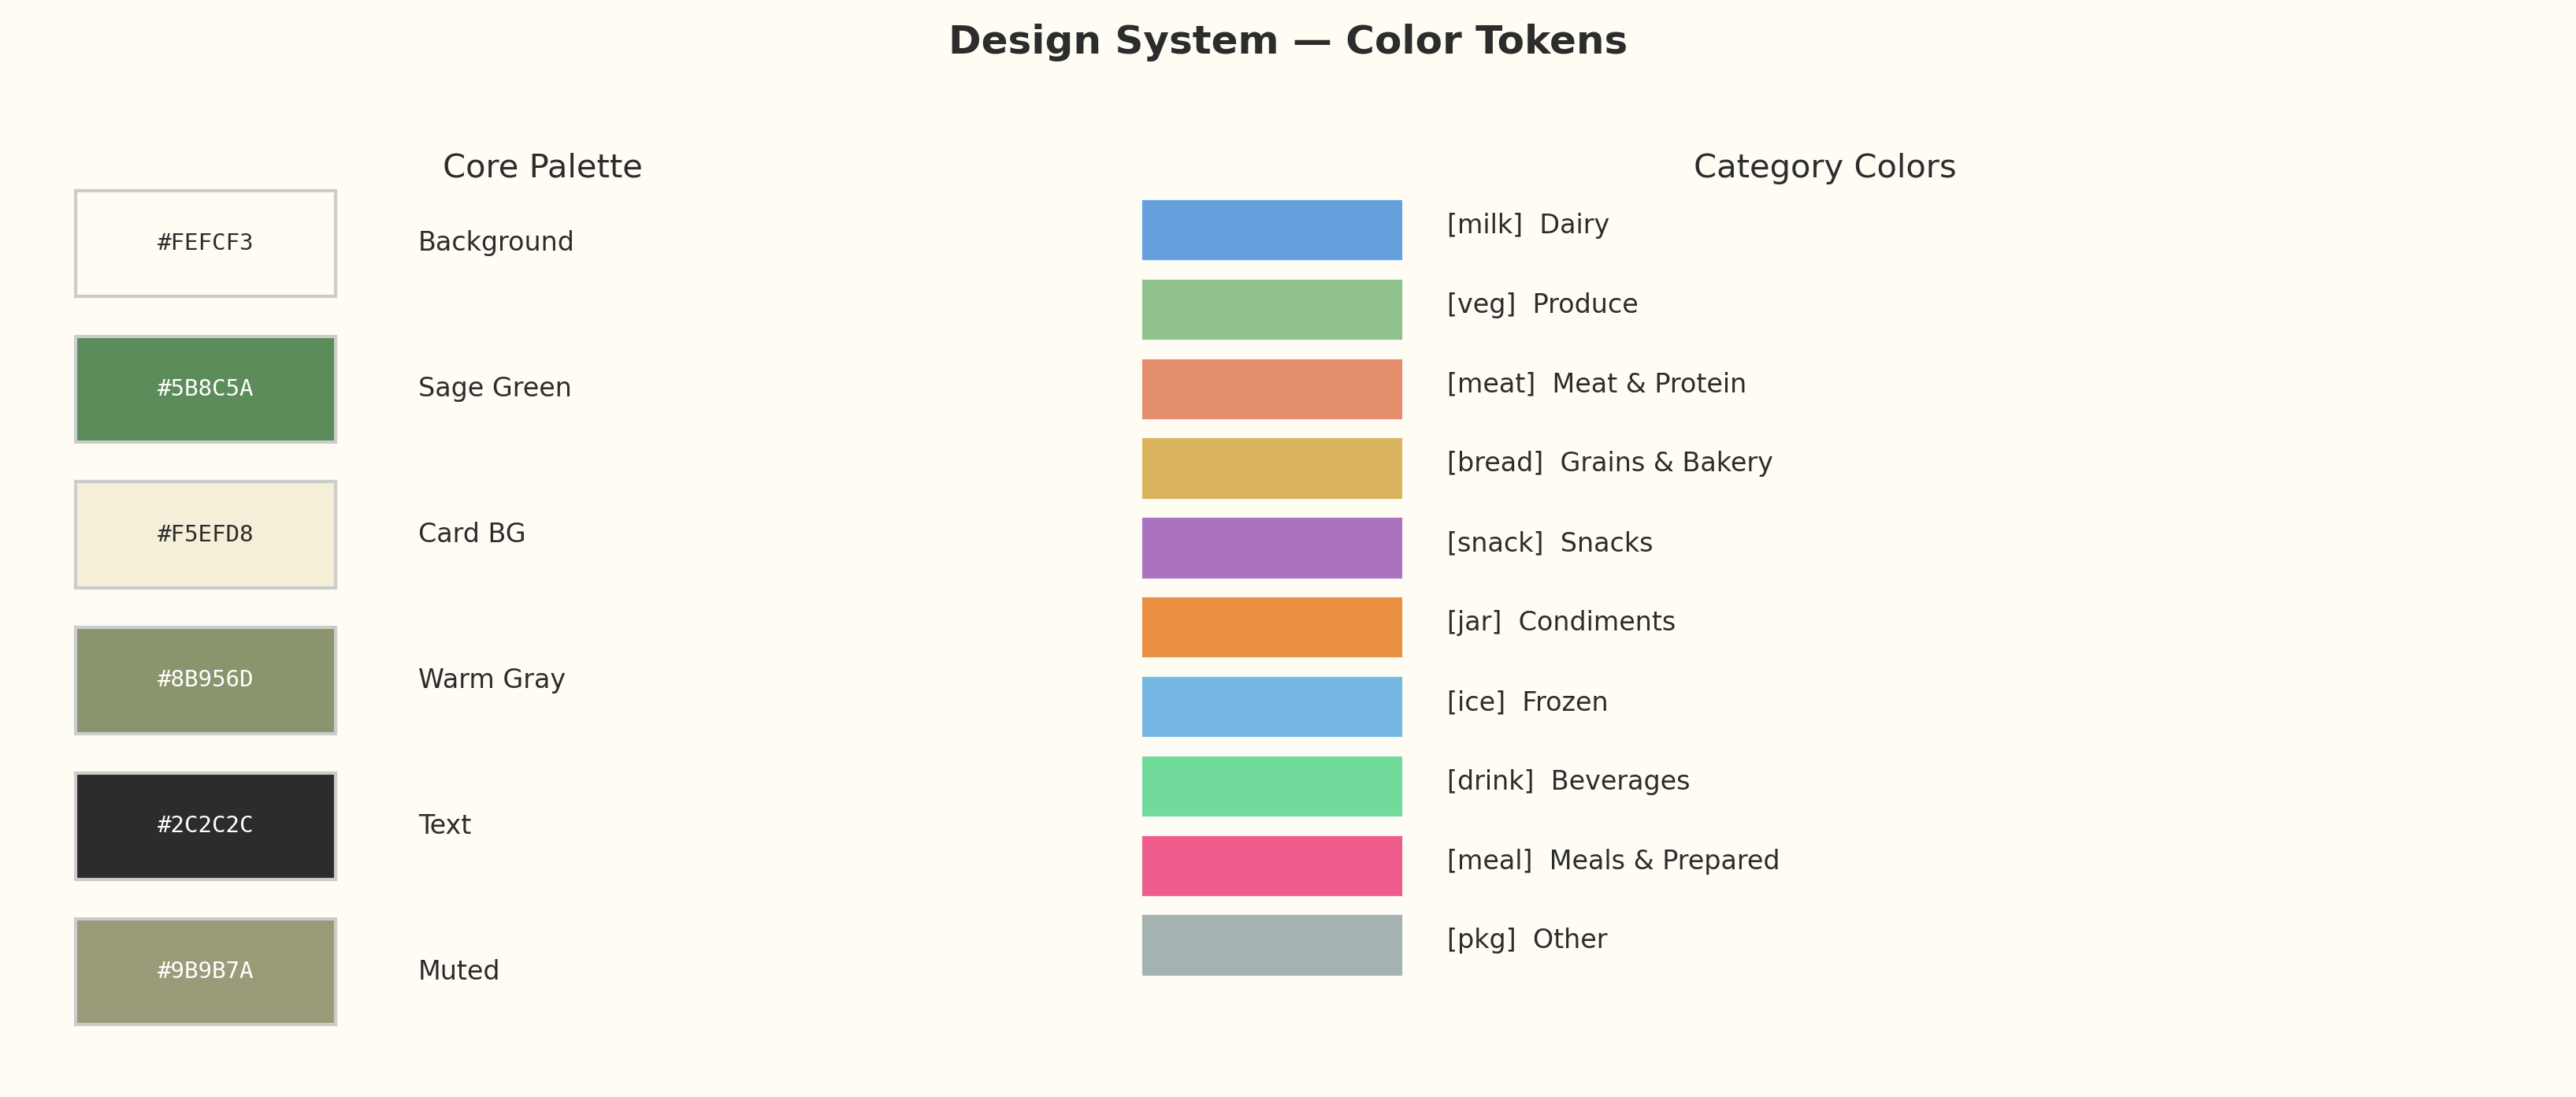
\includegraphics[width=\textwidth]{figures/design_system.png}

    \column{0.44\textwidth}
      \begin{tcolorbox}[pantrybox,title={Typography}]
        {\footnotesize
        \begin{itemize}[leftmargin=*,itemsep=2pt]
          \item \textbf{UI font:} System sans-serif stack
          \item \textbf{Base:} 14px body, 16px card names
          \item \textbf{Card header:} 0.95rem semi-bold
          \item \textbf{Badges/pills:} 0.7rem bold, uppercase
          \item \textbf{Sidebar labels:} 0.8rem muted
        \end{itemize}
        }
      \end{tcolorbox}
      \vspace{0.2cm}
      \begin{tcolorbox}[pantrybox,title={Spacing \& Shape}]
        {\footnotesize
        \begin{itemize}[leftmargin=*,itemsep=2pt]
          \item Cards: \codebox{border-radius: 12px}
          \item Pills/badges: \codebox{border-radius: 20px}
          \item Sidebar: \codebox{border-radius: 0} (full height)
          \item Card shadow: \codebox{0 2px 8px rgba(0,0,0,0.06)}
          \item Grid gap: \codebox{16px}
        \end{itemize}
        }
      \end{tcolorbox}
      \vspace{0.1cm}
      {\footnotesize\color{warmGray}
        All CSS uses custom properties (\codebox{--cream}, \codebox{--sage}, \codebox{--cat-dairy}, ...)
        for easy future theming.
      }
  \end{columns}
\end{frame}

% ── SLIDE 11: TECHNICAL DECISIONS ───────────────────────────
\begin{frame}[t,shrink=25]{Technical Decisions}
  \begin{columns}[T]
    \column{0.48\textwidth}
      \begin{tcolorbox}[pantrybox,title={Why Vanilla JS?}]
        {\footnotesize
        \begin{itemize}[leftmargin=*,itemsep=3pt]
          \item No build step --- edit, reload, done
          \item No dependency rot over time
          \item 58 products: DOM manipulation trivially fast
          \item Serve as static file or tiny Python server
          \item Any LLM can read/edit the whole thing in context
        \end{itemize}
        }
      \end{tcolorbox}
      \vspace{0.2cm}
      \begin{tcolorbox}[pantrybox,title={Why Single-File HTML?}]
        {\footnotesize
        \begin{itemize}[leftmargin=*,itemsep=3pt]
          \item One file = one deploy artifact
          \item No asset pipeline, no CDN needed
          \item Trivial to version in git
          \item Dashboard is a personal tool, not a product --- simplicity wins
        \end{itemize}
        }
      \end{tcolorbox}

    \column{0.49\textwidth}
      \begin{tcolorbox}[pantrybox,title={Build-Eval-Iterate Workflow}]
        {\footnotesize
        \begin{enumerate}[leftmargin=*,itemsep=4pt,label=\textbf{\arabic*.}]
          \item Write full phase spec before building
          \item Builder agent implements the phase
          \item Evaluator agent takes Playwright screenshots at 320/420/768/1200/1920px
          \item Score each spec requirement: Pass / Partial / Fail
          \item Iterate until 100\% match
          \item Gate to next phase
        \end{enumerate}
        \vspace{4pt}
        \textbf{Key insight:} separate builder from evaluator --- different optimization targets.
        Builder optimizes for shipping; evaluator for spec compliance.
        }
      \end{tcolorbox}
      \vspace{0.2cm}
      {\footnotesize\color{warmGray}
        Playwright used headless on server (no display required):\\
        \codebox{npx playwright install chromium}
      }
  \end{columns}
\end{frame}

% ── SLIDE 12: RESULTS ───────────────────────────────────────
\begin{frame}[t,shrink=25]{Results --- 5 Phases, 100\% Spec Match}
  \begin{center}
    \includegraphics[width=0.9\textwidth,height=2.0cm,keepaspectratio]%
      {figures/phases.png}
  \end{center}
  \vspace{0.15cm}
  \begin{columns}[T]
    \column{0.48\textwidth}
      \begin{tcolorbox}[pantrybox,title={What Changed}]
        {\footnotesize
        \begin{itemize}[leftmargin=*,itemsep=1pt]
          \item 10-category system (auto + manual override)
          \item 280px sticky sidebar + hamburger on tablet
          \item Category badges on every card (colored pills)
          \item Location dropdown (replaces blind cycling)
          \item Sort direction toggle (A\textrightarrow{}Z / Z\textrightarrow{}A)
          \item Stats as clickable filters
          \item Skeleton + empty + error states
          \item Out-of-stock badge at qty=0
          \item Null nutrition fields hidden
        \end{itemize}
        }
      \end{tcolorbox}

    \column{0.49\textwidth}
      \begin{center}
        \includegraphics[width=0.95\textwidth,height=3.8cm,keepaspectratio]%
          {figures/phase4-desktop.png}\\[0.05cm]
        {\tiny\color{muted} Phase 4 final --- desktop at 1200px}
      \end{center}
  \end{columns}
\end{frame}

% ── SLIDE 13: WHAT'S NEXT ───────────────────────────────────
\begin{frame}[t,shrink=25]{What's Next --- v3 Roadmap}
  \begin{columns}[T]
    \column{0.33\textwidth}
      \begin{tcolorbox}[pantrybox,title={Nutrition Enrichment}]
        {\footnotesize
        Integrate USDA FoodData Central as fallback \#1 in \codebox{scan.py}.
        Add Spoonacular as fallback \#2.\\[4pt]
        Target: eliminate null nutrition fields for US branded products.\\[4pt]
        \textbf{Effort:} 1 sprint. API keys already identified, both free.
        }
      \end{tcolorbox}

    \column{0.33\textwidth}
      \begin{tcolorbox}[pantrybox,title={Recipe Database}]
        {\footnotesize
        Connect current inventory to a recipe API (Edamam or Spoonacular).\\[4pt]
        Given \{items in pantry\} \textrightarrow{} suggest recipes that use them.\\[4pt]
        Display in new ``Recipes'' tab on dashboard.\\[4pt]
        \textbf{Effort:} 2 sprints. Requires recipe API integration.
        }
      \end{tcolorbox}

    \column{0.31\textwidth}
      \begin{tcolorbox}[pantrybox,title={Shopping List}]
        {\footnotesize
        Track items that hit qty=0 (out of stock).\\[4pt]
        Auto-generate shopping list from out-of-stock + low-stock items.\\[4pt]
        Export as shareable link or push notification.\\[4pt]
        \textbf{Effort:} 1 sprint. Data already available in \codebox{inventory.json}.
        }
      \end{tcolorbox}
  \end{columns}
  \vspace{0.4cm}
  \begin{center}
    \begin{tcolorbox}[colback=cardBg,colframe=sage,boxrule=0.8pt,arc=5pt,
        left=10pt,right=10pt,top=5pt,bottom=5pt,width=0.85\textwidth]
      {\small\color{bodyText}
        \textbf{Stack remains:} single-file HTML + vanilla JS + Python server.
        No framework migration planned.
        Every new feature will follow the same Build-Eval-Iterate pattern with
        explicit spec before implementation.
      }
    \end{tcolorbox}
  \end{center}
\end{frame}

\end{document}
